\chapter{Digital Filter}\label{chap:digitalFilter}

When utilizing a sensor unwanted noise can arise and influence the measurements acquired. By implementing a filter it is possible to attenuate and/or enhance specific frequency components contained in the measurements. When the magnetometer, described in \secref{HardwareChoice}, is active while the vehicle is stationary, the measured angle varies approximately two degrees, see \figref{fig:StationaryMeasurementsMagnato}. The noise affecting the measurements can have a inexpedient effect on the controller which is implemented on the prototype. With ideal circumstances the magnetometer would measure an angle variation of zero degrees. Since this is not the case, implementing a filter to attenuate some of the noise could be a potential solution to get more accuracy.

There is many cons and pros when considering between implementing a analogue or digital filter. For example a analogue filter only utilizes hardware and therefore does not occupy as much of the computation time on the microprocessor as a digital filter. On the other hand since the analogue filter utillized component's it is exposed to component tolerances. Besides the microprocessor a digital filter will need no components, since the data received from the magnetometer is already digitalized.

From these few arguments it has been chosen to implement a digital filter, since the signal received from the magnetometer has already been digitalized, and it would therefore be impractical to implement an analogue filter.

In the following point form the separate sections in this chapter are illustrated. The point form has been made to make the overall steps when designing a filter more clear to the reader.

\begin{itemize}
\item Frequency analysis of measured data
\item Specific requirements
\item Filter type
\item Design
\item Implementation
\item Results
\end{itemize}

When designing and implementing a filter a few considerations needs to be made first. In the first section the measured data will be frequency analysed to give a base for creating requirements for the filter. After making specific requirements for the filter it is possible to examine and decide which filter would be suitable for fulfilling the requirements, without influencing the desired frequencies. Hereafter, it is possible to design and implement the filter, and thereafter conclude if the filter complies with what is desired.

The following section contains a frequency analysis of the measured data which is need to set up requirement for the filter.

\section{Frequency Analysis of Measured Data}
Before designing a filter it is necessary to analyse data measured with the magnetometer, to ensure the signal is not attenuate and as must noise is removed (attenuated) as possible. The data analysed is when the vehicle and the magneto is stationary, and thereby finding the stationary variations on the sensor, the acquired measurements is illustrated in \figref{fig:StationaryMeasurementsMagnato}.

\begin{figure}[H]
  \centering
 	%Trim margins @:   left        bottom       right       top
 	\adjustbox{ trim = {.15\width} {.30\height} {.15\width} {.30\height}, clip }
  {
    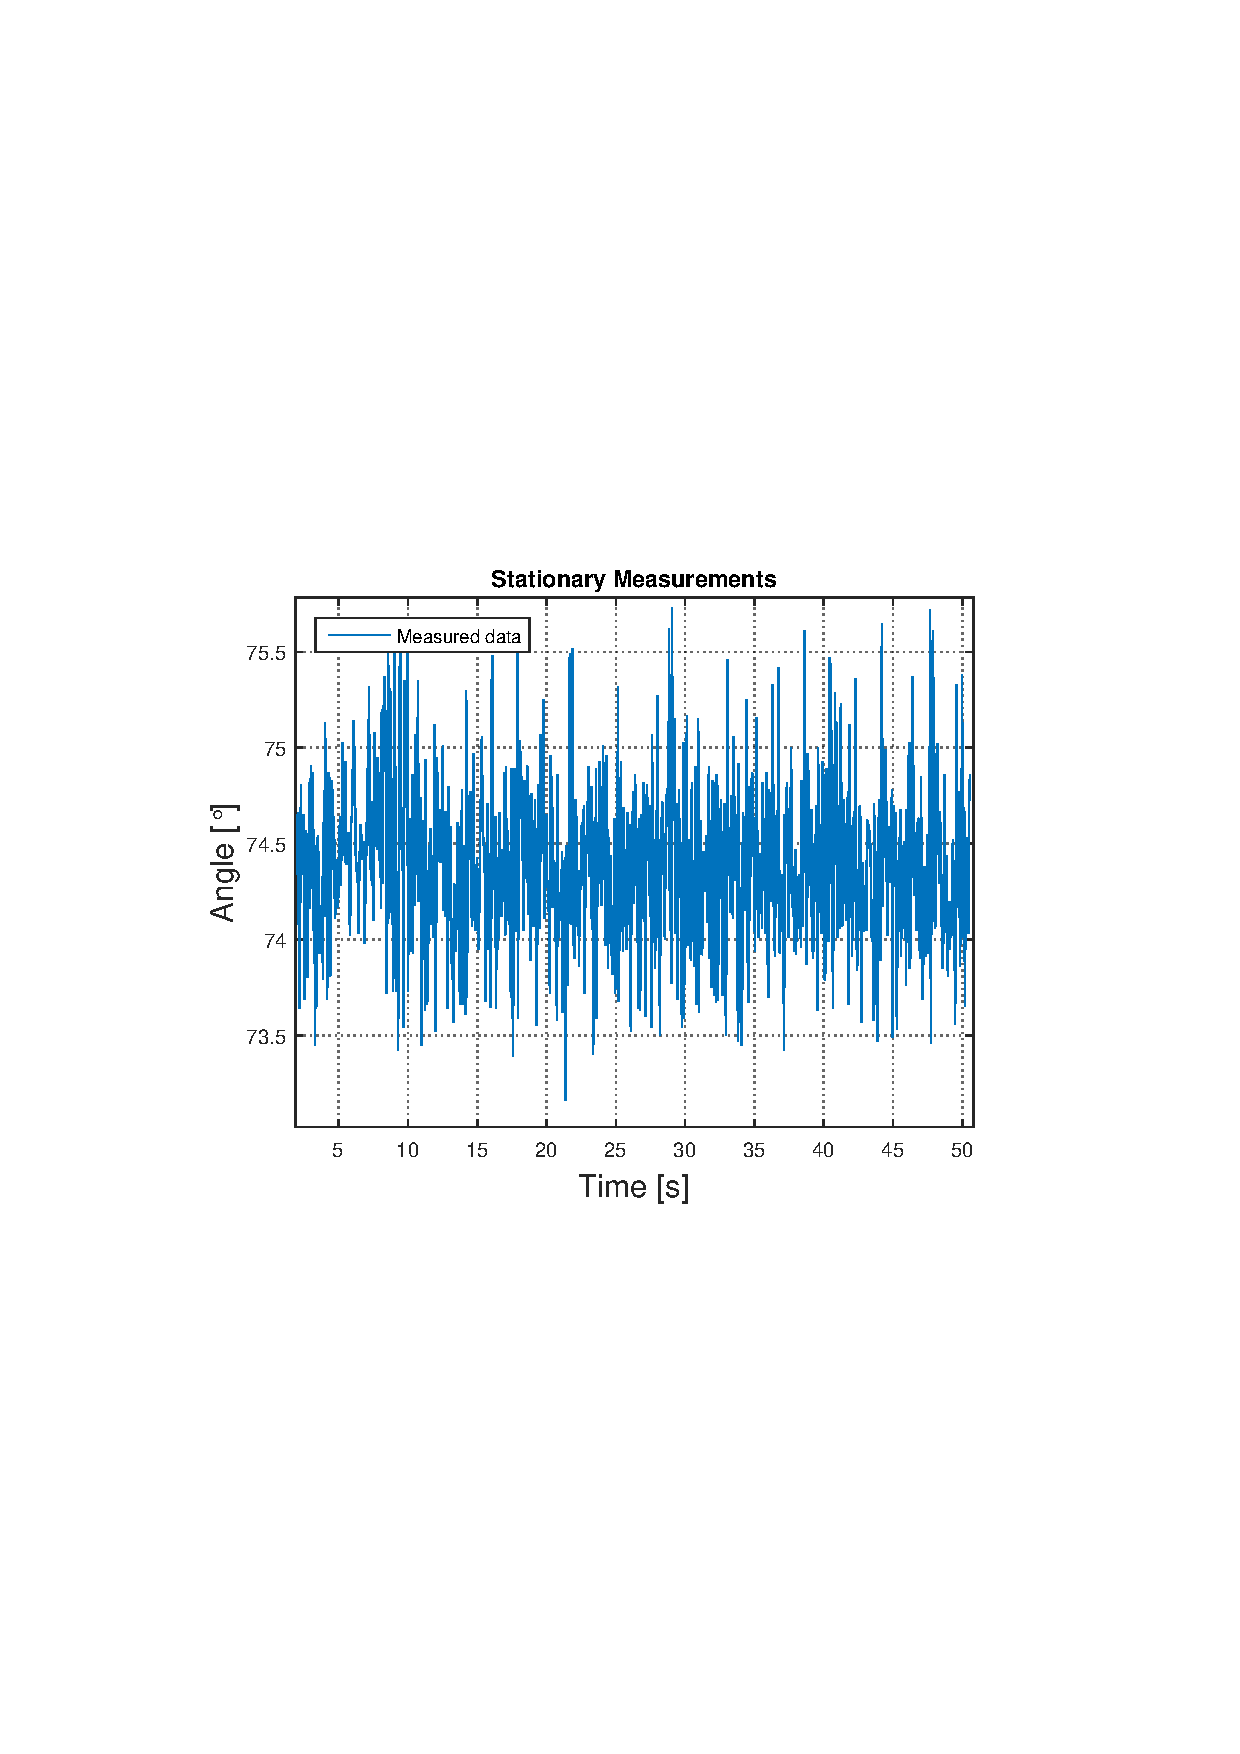
\includegraphics[width=1.1\textwidth]{figures/StationaryMeasurementsMagnato.pdf}
  }
  \caption{A plot, where the x-axis is time and the y-axis is the angle, of data measured with the magnetometer while the vehicle is stationary.}
  \label{fig:StationaryMeasurementsMagnato}
\end{figure}

From \figref{fig:StationaryMeasurementsMagnato} it can be seen how the angle measured vary with approximately 2 degrees. In the datasheet for the magnetometer it is explained that the sensor has a 1 to 2 degrees accuracy \cite{MagnoDatasheet}, which is consistent with the measured data. To be able to analyse measured data affected by noise, a FFT is utilized to convert the signal from time-domain to frequency domain. The FFT makes it possible to see the frequency component contained in the signal, thereby making it possible to find the signal and the noise affecting the signal. A FFT of the measured data is performed and illustrated in \figref{fig:StationaryMeasurementsMagnato}.

\begin{figure}[H]
  \centering
 	%Trim margins @:   left        bottom       right       top
 	\adjustbox{ trim = {.15\width} {.30\height} {.15\width} {.30\height}, clip }
  {
    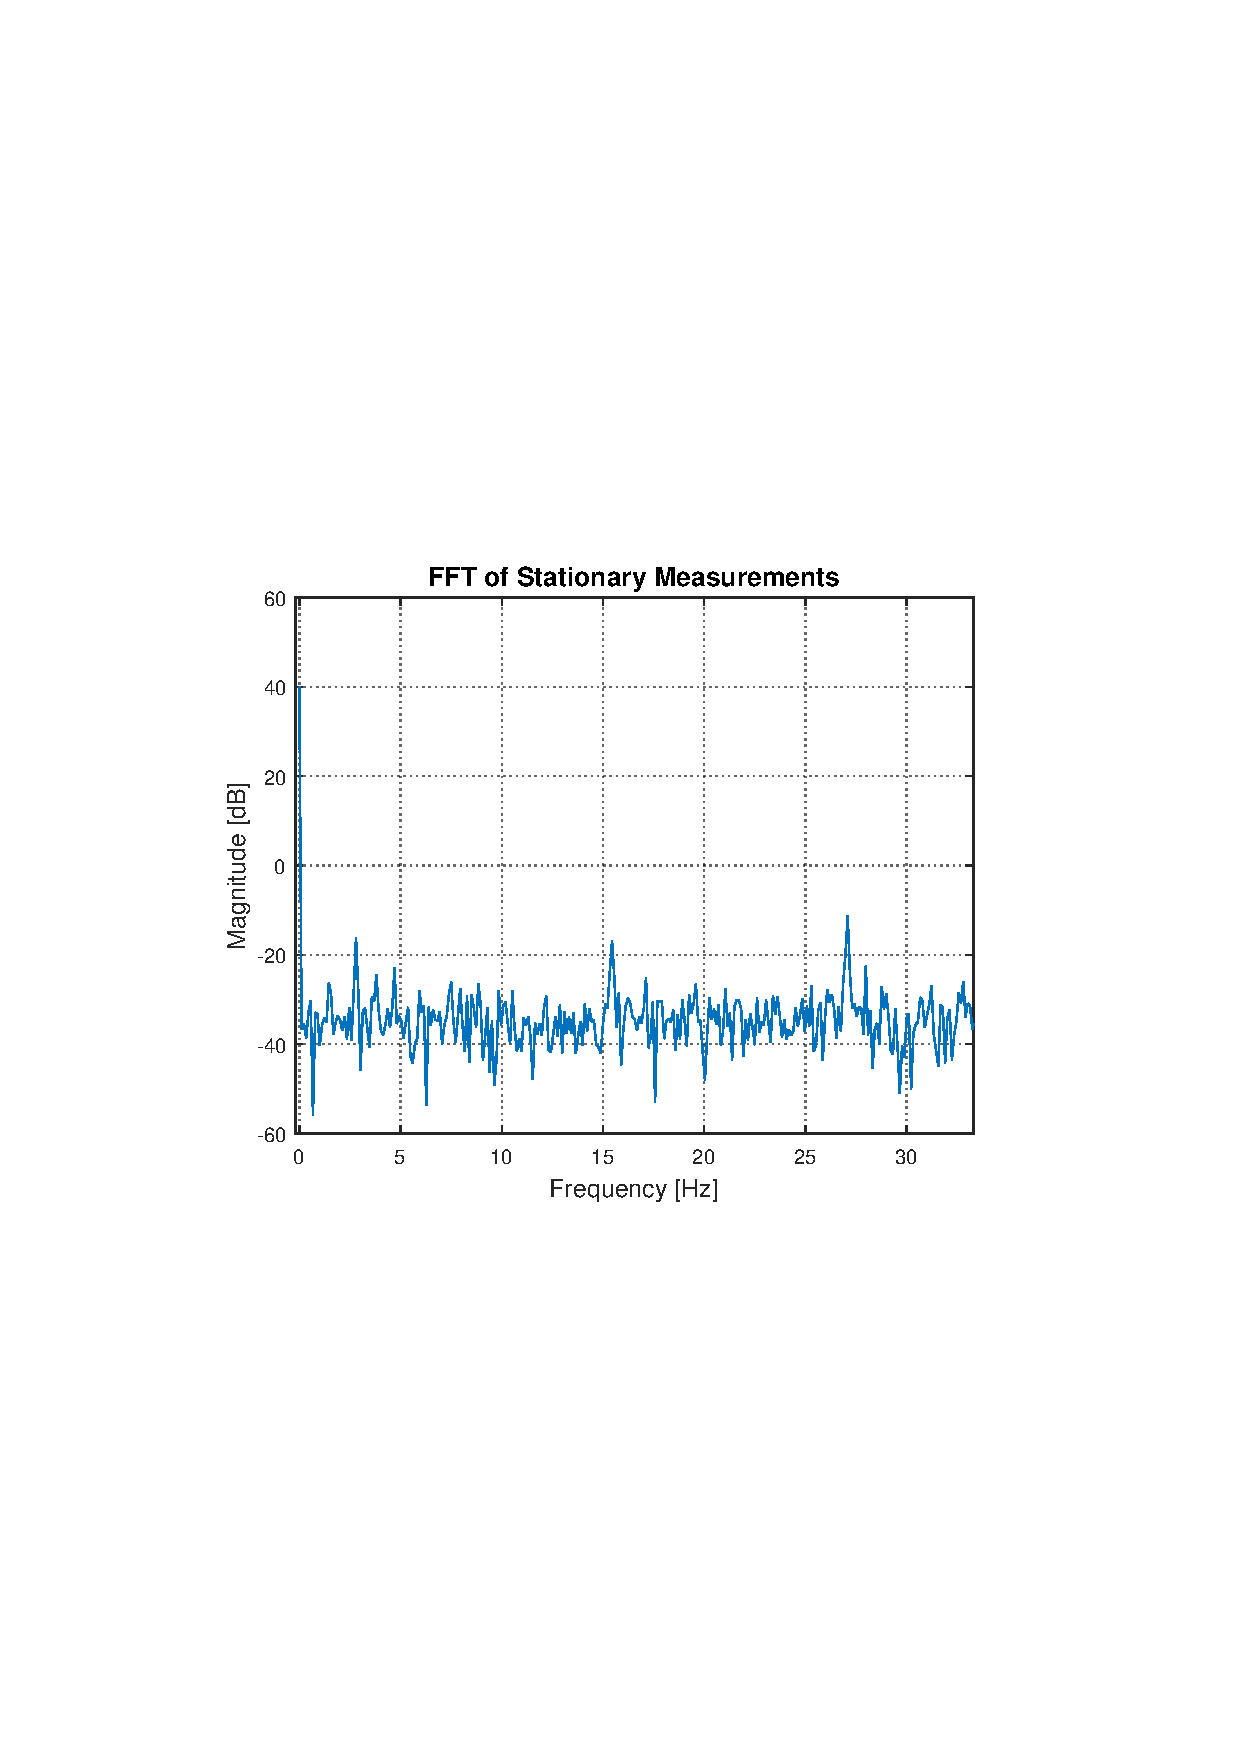
\includegraphics[width=1.1\textwidth]{figures/FFTofStationaryMeasurements.pdf}
  }
  \caption{A FFT of the measured data illustrated in \figref{fig:StationaryMeasurementsMagnato}}
  \label{fig:FFTofStationaryMeasurements}
\end{figure}

The data measured in \figref{fig:StationaryMeasurementsMagnato} is acquired with a sampling frequency of 40 \si{Hz}. The Nyquist-Shannon Sampling Theorem says that to find the frequency components contained in a signal you need atleast twice the sampling frequency \cite{AVOppenheim}:
%
\begin{flalign}
\Omega_s &\geq 2 \cdot \Omega_N \unit{Hz}
\end{flalign}
\hspace{6mm} Where:\\
\begin{tabular}{p{1cm}lll}
& \si{\Omega_s}            	& is the sampling frequency         &\unitWh{Hz} \\
& \si{\Omega_N}				& is the Nyquist frequency			&\unitWh{Hz} \\
\end{tabular}

This is illustrated in \figref{fig:FFTofStationaryMeasurements}, where the frequency components only goes from 0 to 20 Hz on the x-axis, which is half the sampling frequency. The y-axis is the magnitude of the frequency component, measured in \si{dB}, occurring in the signal.

From the FFT performed, seen in \figref{fig:FFTofStationaryMeasurements}, a spike is present at 1 \si{Hz}, this is the DC value, i.e. the offset seen in \figref{fig:StationaryMeasurementsMagnato}. This frequency component is the signal which the filter should not attenuate. The frequency components present after 1 Hz and to 20 Hz, is the noise from the sensor, and is what is desired to filter. 

Some consideration has to be made for the filter requirements, to ensure that the filter is not influencing the system and the desired frequency needlessly.

\section{Filter Requirements} \label{sec:FilterRequirements}
Before selecting which filter to design and implement, it is necessary to examine requirements needed for performing the necessary filtering. These requirements will be found by using the FFT, which is plotted in previous section, and by looking at the sample rate for the internal loop in the steering model, see \secref{sec:}. 

Since it is desired to influence the DC-signal as little as possible a low-pass filter is implemented. The ideal filter will have a passband attenuation of 0 \si{dB}, since this is not a ideal filter a maximum attenuation variation is set from 1 \si{dB} to 0 \si{dB}. To ensure the filter is not delaying the signal to much a cut-off frequency of 10 \si{Hz} has been decided. Further more it has been decided to have 40 \si{dB} attenuation at 17 \si{Hz}.
 
To convert from the specifications in continuous-time to specification for a discrete-time filter, the relationship between continuous- and discrete-time is utilized:

\begin{flalign}
\eq{\omega}{\Omega \cdot T_s}
\end{flalign}

The filters discrete-time specification is therefore:

\textbf{Passband specification:}
\begin{flalign}
0.89125 &\leq |H(e^{j\omega}| \leq 1 \\
0 &\leq \omega \leq 0.3\pi
\end{flalign}

\textbf{Stopband specification:}
\begin{flalign}
|H(e^{j\omega})| &\leq 0.01 \\
0.3 &\leq \omega \leq \pi
\end{flalign}

\section{Filter Type}
The specification for the filter is set and it is possible to examine which filter would be suitable for fulfilling the specified requirements, without influencing the DC-value and the system needlessly.

\begin{figure}[H]
	\centering
	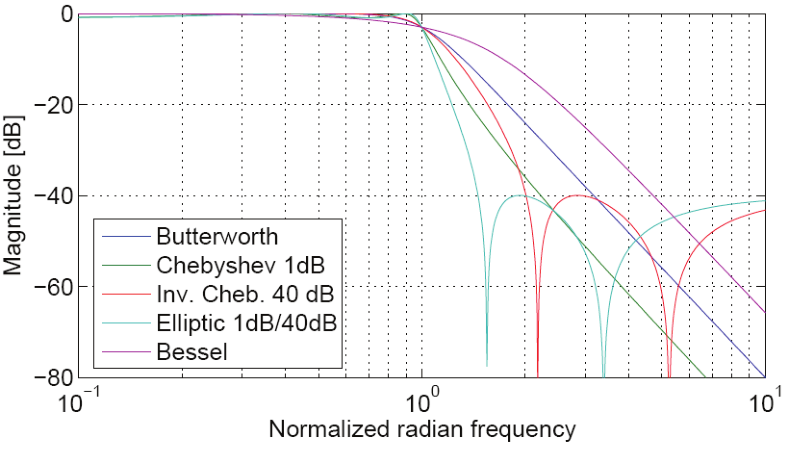
\includegraphics[scale=1]{figures/Filtertypes1.pdf}
	\caption{Frequency response for various filter types}
	\label{fig:Filtertype1}
\end{figure}

The disadvantages of a Elliptic filter is that it has both ripples in the pass- and stopband. additionally, it has a high group delay both before and at the cutoff frequency, this can be seen in \figref{fig:groupdelay}. The advantage of a Elliptic filter is that is has the sharpest cut-off frequency of the filters illustrated in \figref{fig:Filtertype1}.

The Chebyshev filter only has ripples in the passband, and a sharp cut-off frequency, but still has a high group delay before and at the cut-off frequency. The inverse Chebyshev only has ripples in the stopband, but does not have as sharp cut-off frequency as the Chebyshev and the Elliptic filter. Compared to the two former filter it has a lot less group delay before and after the cut-off frequency.

The Bessel filter has the lowest group delay before and at the cut-off frequency, see \figref{fig:groupdelay}. additionally, it does not have any ripples, neither in pass- or stopband. The disadvantage of the filter is it has the least sharpest cut-off frequency of the filters illustrated in \figref{fig:Filtertype1}.

The Butterworth filter has a sharper cut-off frequency compared to the Bessel filter and as the Bessel filter it does not have any ripples neither in the pass- or stopband. Furhtermore, the Butterworth filter has the second lowest group delay at the cut-off frequency compared to the other filters illustrated in \figref{fig:groupdelay}. 

\begin{figure}[H]
	\centering
	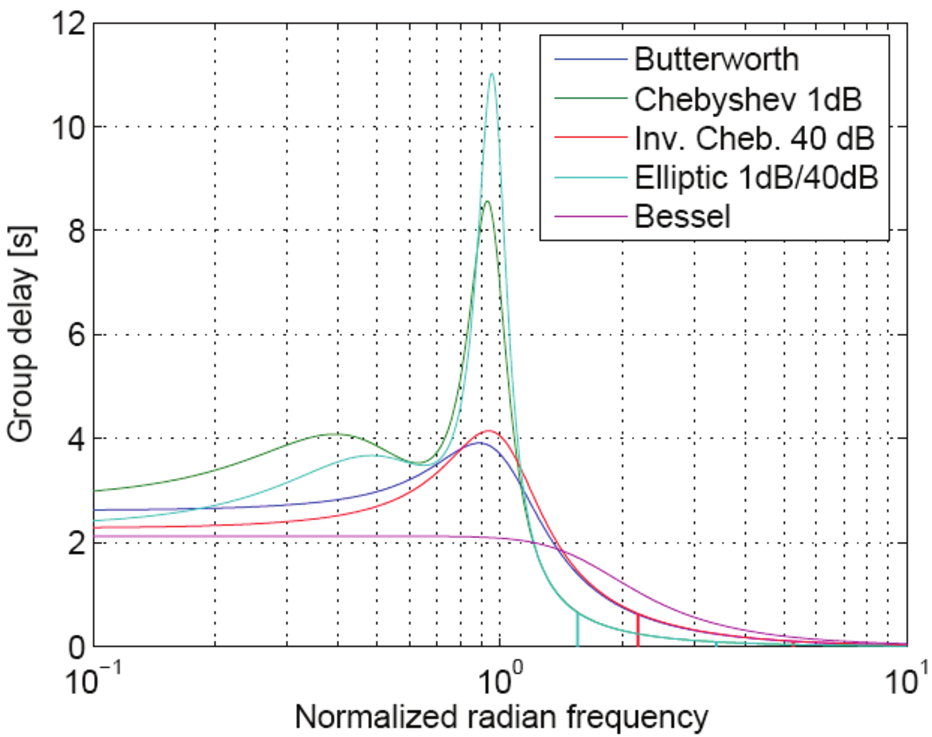
\includegraphics[scale=0.7]{figures/Filtertypes2.pdf}
	\caption{Frequency response illustrating group delay for various filter types}
	\label{fig:groupdelay}
\end{figure}

Because of the above-mentioned descriptions of the filter a Butterworth filter has been selected for filtering the measured data. The Butterworth does not have any ripples in the passband which could influence the DC-value, seen in \figref{fig:FFTofStationaryMeasurements}, and it upholds the requirement set for the filter in \secref{sec:FilterRequirements}. Compared to the other described filters, the Butterworth has a small group delay.

The requirements and filter type has been chosen, and it is thereby possible to design the filter which has to be implemented.

\section{Design}

\subsection{General transfer function}

Pre-warping: 

\begin{flalign}
\eq{\Omega}{2 \cdot T_d \cdot \tan{\frac{0.3 \pi}{2}}} \\
\end{flalign}

Magnitude squared function:

\begin{flalign}
\eq{|H(e^{j\omega}|^2}{\frac{1}{1+(\frac{\Omega}{\Omega_c})^{2N}}} \\
\end{flalign}

Poles:

\begin{flalign}
\eq{P_k}{\Omega_c \cdot e^{j(\frac{2 \cdot k -1}{2 \cdot N} \cdot \pi + \frac{\pi}{2})}} \\
\eq{k}{1,2 \dotsc N}
\end{flalign}

General transfer function:

\begin{flalign}
\eq{H(s)}{\frac{G_o}{\prod\limits_{k = 1}^N (s-P_k)}}
\end{flalign}

Transfer function:

\begin{flalign}
\eq{H(s)}{\frac{G_o}{(s-e^{j\cdot \frac{2}{3} \cdot \pi})}}
\end{flalign}

The next step would be to transfer the continuous-time Butterworth filter to the z-domain.

\subsection{Bilinear Transform vs. Impulse Invariance transformation}
Before transferring a continuous-time filter to the z-domain, the two most common transformation methods is examined.

\textbf{Bilinear transform} is 

\begin{figure}[H]
	\setcounter{subfigure}{0}
	\centering
	\begin{subfigure}{.45\textwidth}
		\centering
		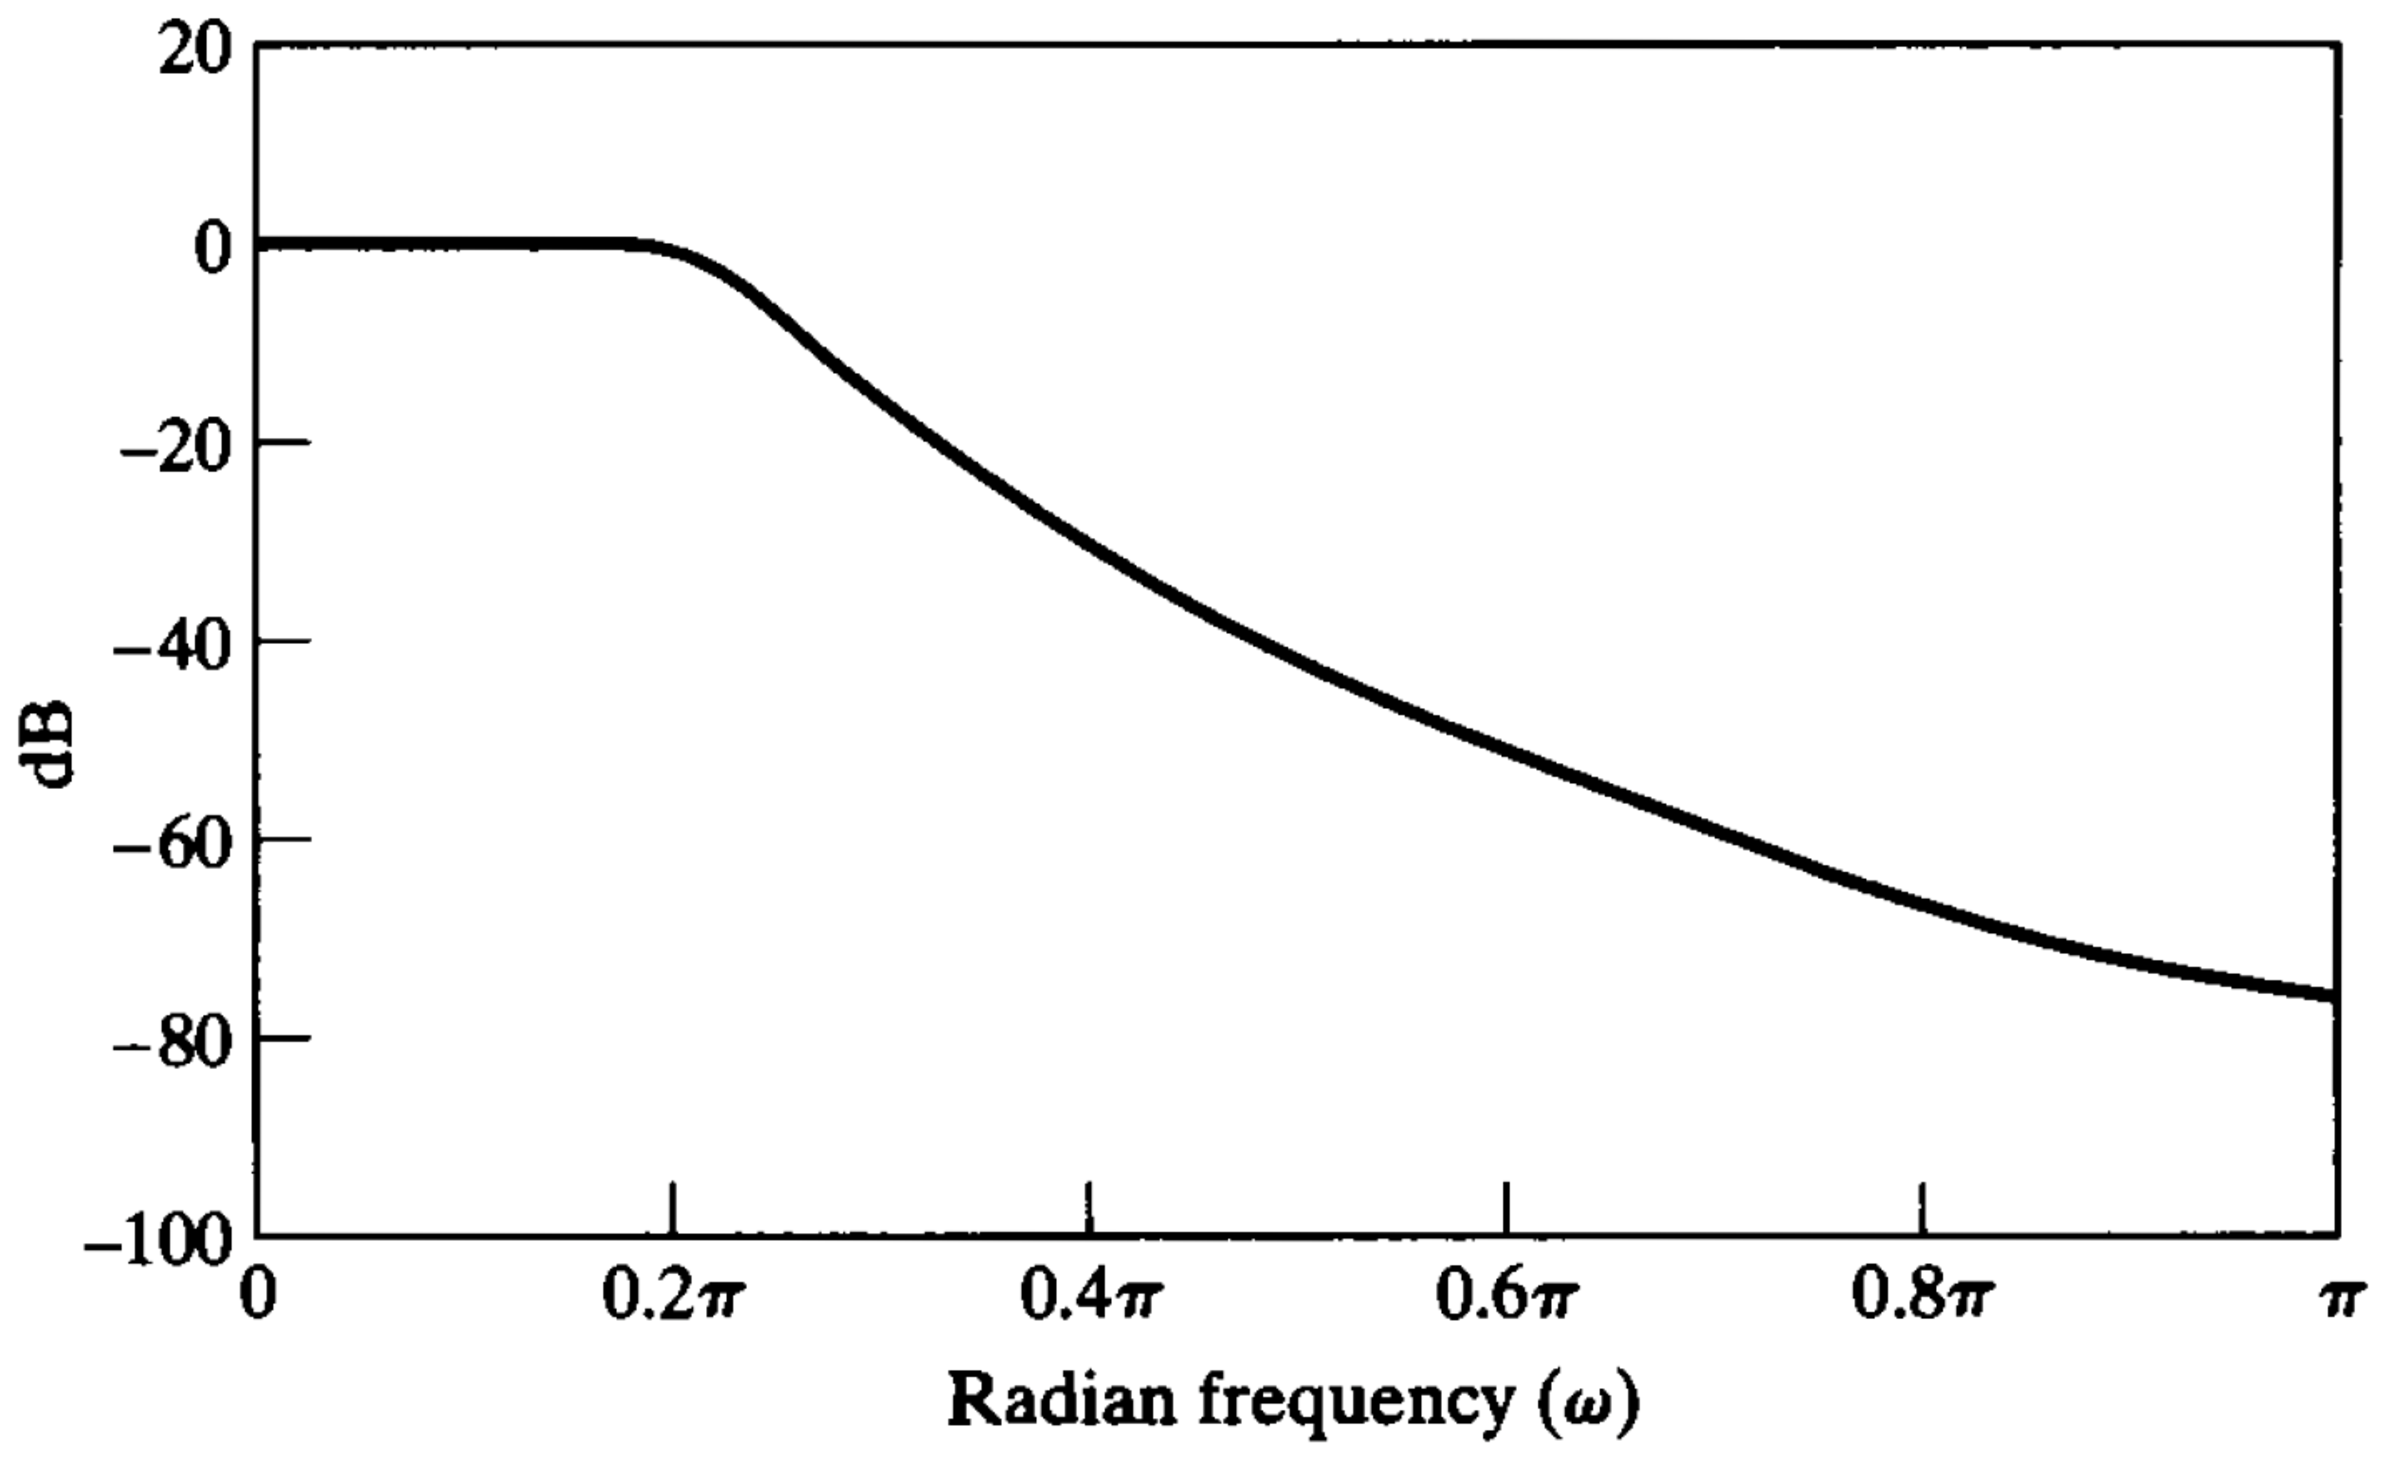
\includegraphics[width=\linewidth]{figures/BilinearFrequencyResponse.pdf}
		\caption{A frequency response of a transformed impulse variance 6th order Butterworth filter}
		\label{fig:ImpulseVarianceResponse}
	\end{subfigure}
	\hfill
	\begin{subfigure}{.45\textwidth}
		\centering
		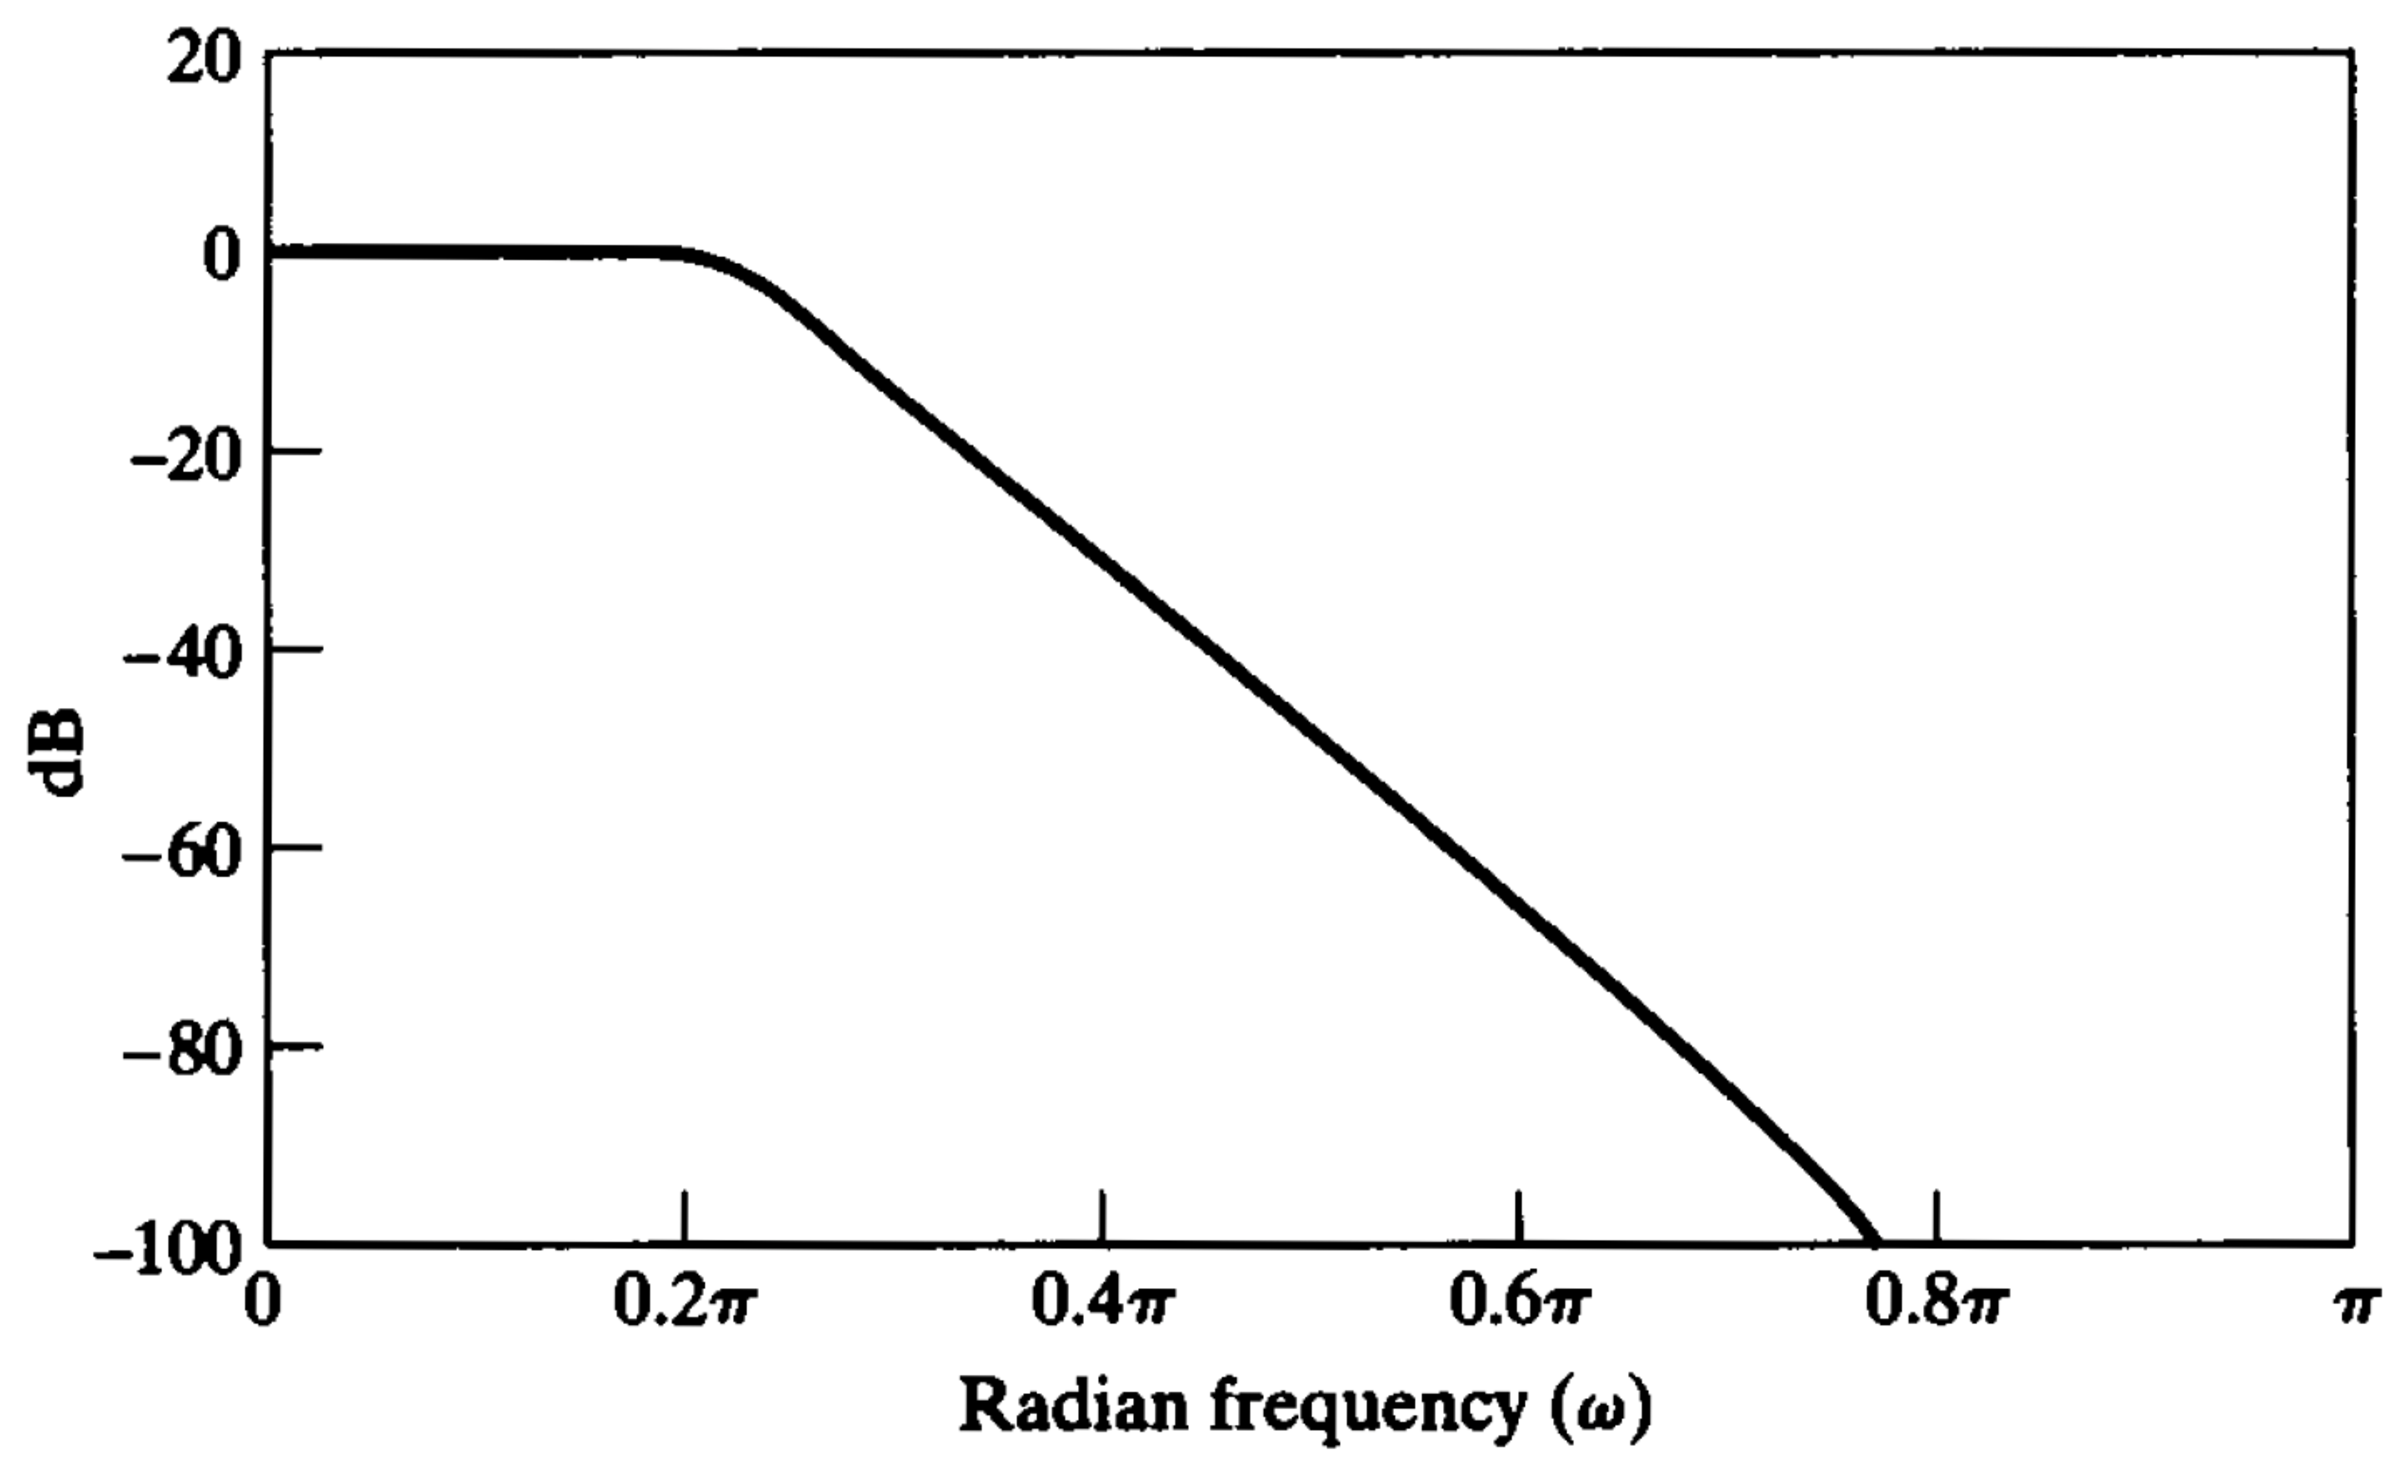
\includegraphics[width=\linewidth]{figures/ImpulseVariantFrequencyResponse.pdf}
		\caption{A frequency response of a transformed bilinear transform 6th order Butterworth filter}
		\label{fig:BilinearTransformResponse}
	\end{subfigure}
	\caption{frequency response of a 6th order Butterworth filter, transformed from continuous time to the z-domain by two different methods named Bilinear transform and Impulse Variance}
		\label{fig:bilinearandimpulsevariance}
\end{figure}

\subsection{Transforming the filter to Z-domain}


Standard formula:

\begin{flalign}
H(z) &= \frac{B(z)}{A(z)} = \frac{b_0 + b_1z^-1 + b_2z^-2 + \dotsc + b_Nz^{-N}}{1 + a_1z^-1 + a_2z^-2 + \dotsc + a_Mz^{-M}}
\end{flalign}

\section{Implementation}

\subsubsection{Direct Form I}

\subsubsection{Direct Form II}

\section{Results}